\documentclass[12pt,a4paper]{article}
\usepackage[spanish]{babel}
\usepackage[utf8]{inputenc}
\usepackage[T1]{fontenc}
\usepackage{lmodern}
\usepackage{geometry}
\geometry{margin=2.5cm}

\usepackage{graphicx}
\usepackage{float}
\usepackage{subcaption}
\usepackage{wrapfig}
\usepackage{tcolorbox}
\usepackage{url}
\usepackage{hyperref}
\hypersetup{
colorlinks=true,
linkcolor=black,
urlcolor=blue,
citecolor=black
}

\tcbset{
colback=gray!10,
colframe=black,
boxrule=0.8pt,
arc=4pt,
left=6pt,
right=6pt,
top=6pt,
bottom=6pt
}

\newcommand{\volverindice}{
\vspace{0.3cm}
\begin{flushright}
\small\hyperlink{indice}{\textit{Volver al índice}}
\end{flushright}
}

\title{Módulos Odoo – Modelos y Vistas}
\author{Birhan Fdez}
\date{22 de abril de 2026}

\begin{document}

\maketitle

\begin{figure}[H]
\centering

\includegraphics[width=1\textwidth]{Img/odoo_logo.png}
\end{figure}

\newpage
\hypertarget{indice}{}
\tableofcontents

\newpage
\volverindice
\section{Introducción}
En este documento se presenta una guía detallada sobre el desarrollo de las actividades de la \textbf{Práctica 4 del modelo de Odoo}.

El objetivo principal de esta práctica es aplicar los conocimientos adquiridos sobre los modelos relacionales y vistas a la hora de desarrollar aplicaciones en el entorno de Odoo. Para ello, implementaremos los distintos módulos que abarcan la gestión de tareas, la gestión de pacientes, médico y consultas en un hospital, la organización de ciclos formativos en un instituto y la gestión de una biblioteca de cómics.

Esta práctica pretende que el usuario comprenda la interacción de los módulos, sus relaciones y sus vistas, además de su integración con las interfaces de \textbf{Odoo} para la gestión de información.

\section{Consideraciones previas}
Antes de comenzar con las actividades, será necesario realizar una serie de pasos previos.

Lo primero que se debe hacer es acceder al repositorio de GitHub donde se encuentran los módulos de ejemplo proporcionados.

\textbf{https://github.com/sergarb1/OdooModulosEjemplos}

Una vez dentro del repositorio, procederemos a descargar los módulos presentes en formato \textbf{.ZIP}.

\begin{figure}[H]
\centering
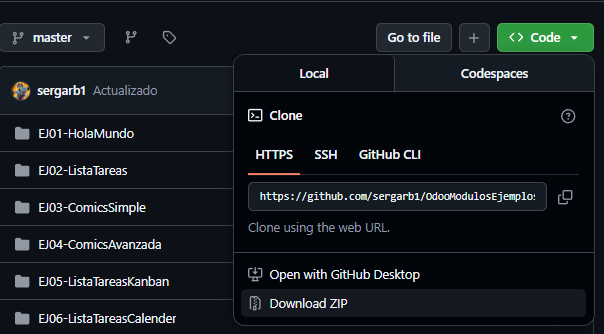
\includegraphics[width=1\textwidth]{Img/od0.png}
\end{figure}

\newpage
\volverindice
Tras finalizar la descarga, añadiremos los módulos dentro de la carpeta \textbf{Addons} del entorno de Odoo para su uso en las actividades.

\begin{figure}[H]
\centering
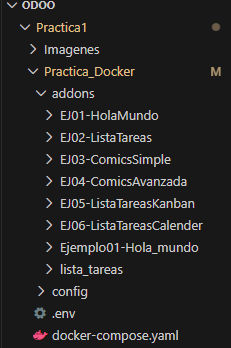
\includegraphics[width=0.5\textwidth]{Img/od1.png}
\end{figure}

Con los módulos añadidos, nos dirigiremos a Odoo para realizar una actualización de la lista de aplicaciones utilizando los permisos de administración. Posteriormente, desde el buscador de aplicaciones, introduciremos el prefijo \textbf{EJ0} para comprobar que los módulos se hayan instalado correctamente.

\begin{figure}[H]
\centering
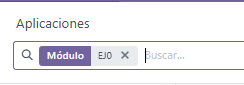
\includegraphics[width=0.6\textwidth]{Img/od.png}
\end{figure}

\begin{figure}[H]
\centering
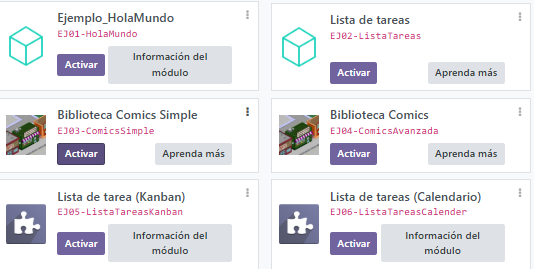
\includegraphics[width=0.8\textwidth]{Img/od3.png}
\end{figure}

Una vez comprobado que los módulos han sido instalados de forma correcta, podremos dar inicio a las actividades principales de esta práctica.

\section{Actividad 01: Modificación de Lista de Tareas}
En esta actividad, se nos pide realizar dos modificaciones sencillas al módulo de \textbf{Lista de Tareas} desarrollado en una práctica anterior.

\subsection{Añadido vista Kanban}
La primera modificación que se nos pide es añadir una nueva vista en formato \textbf{Kanban}. Para ello, debemos dirigirnos al archivo \textbf{views.xml} del módulo en la carpeta \textbf{Views}.

Una vez dentro, debemos agregar el siguiente código para añadir la nueva vista a la lista de tareas.

\begin{figure}[H]
\centering
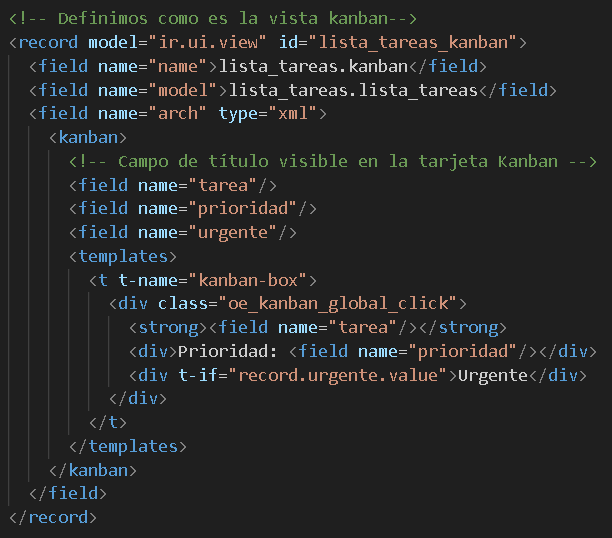
\includegraphics[width=0.7\textwidth]{Img/od01.png}
\end{figure}

\newpage
\volverindice
Con el código principal de la vista añadido, nos dirigiremos al apartado de acciones y menús para activar la nueva vista. Para ello ingresamos el siguiente código:

\begin{figure}[H]
\centering
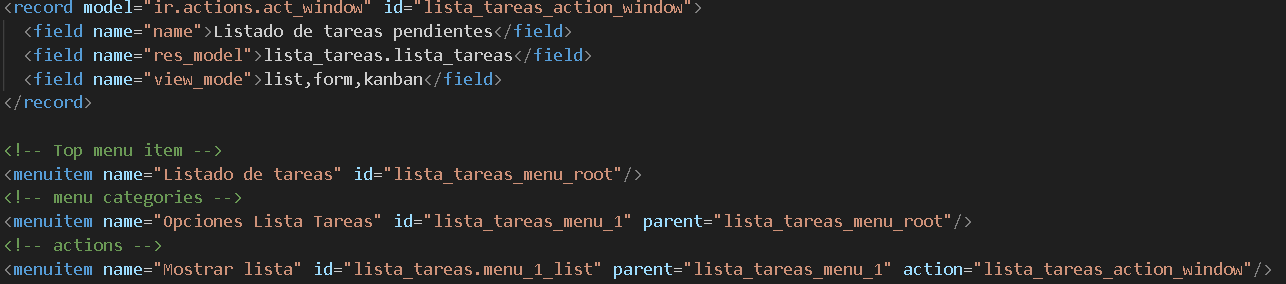
\includegraphics[width=1.1\textwidth]{Img/od03.png}
\end{figure}

\subsection{Nuevo campo y nueva vista Calendario}
Con la vista \textbf{Kanban} añadida, el segundo apartado de la actividad nos pide modificar los campos de las tareas añadiendo el nuevo campo \textbf{fecha asignada}. Esto se realiza desde el archivo \textbf{models.py} en la carpeta \textbf{Models}. Dentro, añadiremos el siguiente campo:

\begin{tcolorbox}[title=Nuevo Campo Fecha]
\begin{verbatim}
fecha_vencimiento = fields.Date(string="Fecha de Vencimiento")
\end{verbatim}
\end{tcolorbox}

Una vez agregado este nuevo campo, la clase lista quedará de esta forma:

\begin{figure}[H]
\centering
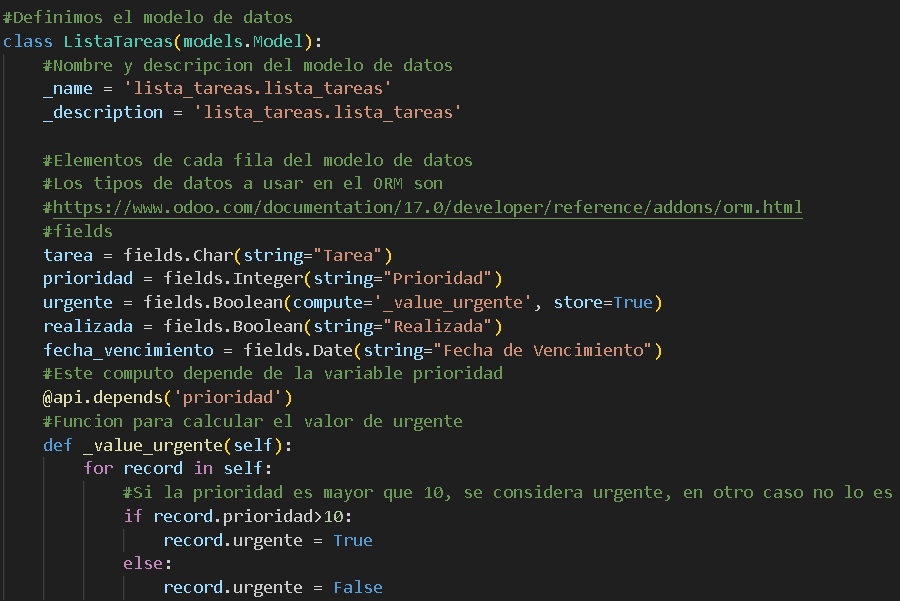
\includegraphics[width=1\textwidth]{Img/od05.png}
\end{figure}

Tras completar la modificación de la clase, nos volveremos a dirigir al \textbf{apartado de vistas}, donde nos pide añadir una vista de calendario así como actualizar el apartado de acciones.

\newpage
\volverindice
Para ello, ingresaremos el siguiente código que gestionará la vista calendario.

\begin{tcolorbox}[title=Nueva Vista Calendario]
\begin{figure}[H]
\centering
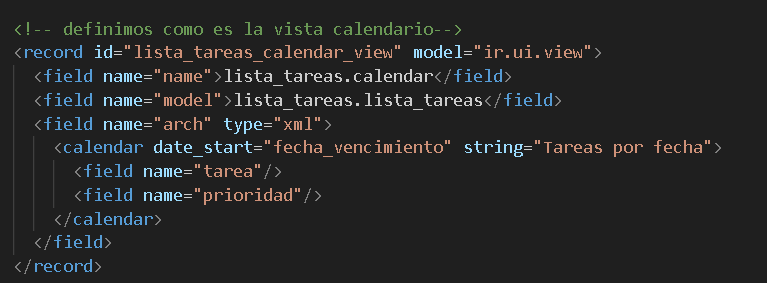
\includegraphics[width=1\textwidth]{Img/od02.png}
\end{figure}
\begin{figure}[H]
\centering
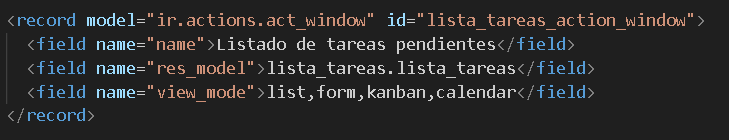
\includegraphics[width=1\textwidth]{Img/od04.png}
\end{figure}
\end{tcolorbox}

\subsection{Comprobación de Vistas}
Con las nuevas modificaciones implementadas en el módulo, realizaremos una comprobación actualizando el módulo y haciendo una prueba.

Para ello, empleando los filtros, localizaremos nuestro módulo \textbf{Lista\_Tareas}. Una vez localizado, lo actualizamos para implementar los nuevos cambios.

\begin{figure}[H]
\centering
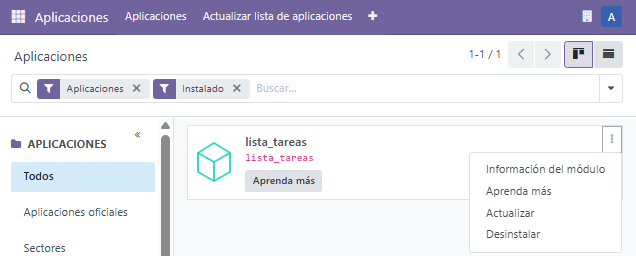
\includegraphics[width=0.8\textwidth]{Img/od6.1.png}
\end{figure}

\newpage
\volverindice
Una vez completada la actualización, ingresaremos al módulo para realizar una prueba cuyo objetivo es confirmar que las modificaciones funcionan correctamente.

\begin{figure}[H]
\centering
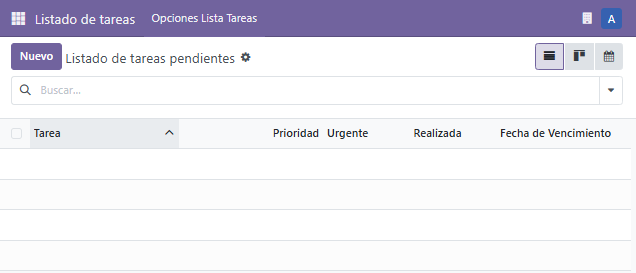
\includegraphics[width=1\textwidth]{Img/od6.png}
\end{figure}

Para ello, crearemos una nueva tarea que incluirá el nuevo campo \textbf{Fecha de Vencimiento}.

\begin{figure}[H]
\centering
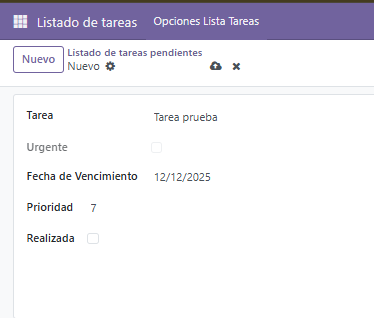
\includegraphics[width=0.8\textwidth]{Img/od7.png}
\end{figure}

\newpage
\volverindice
\begin{figure}[H]
\centering
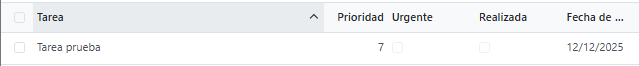
\includegraphics[width=0.8\textwidth]{Img/od8.png}
\end{figure}

Con la nueva tarea de prueba creada, nos dispondremos a navegar por las nuevas vistas observando que no tengamos ningún problema y que están funcionales.

La primera vista que comprobaremos es la vista \textbf{Kanban}.

\begin{figure}[H]
\centering
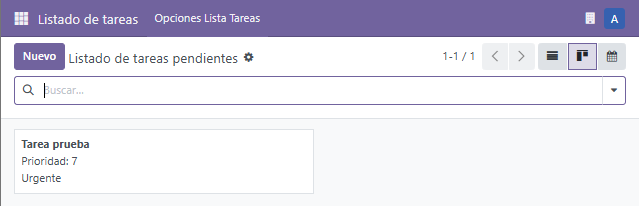
\includegraphics[width=0.8\textwidth]{Img/od10.png}
\end{figure}

Seguido de la vista \textbf{Calendario}, que nos mostrará en la fecha asignada la nueva tarea.

\begin{figure}[H]
\centering
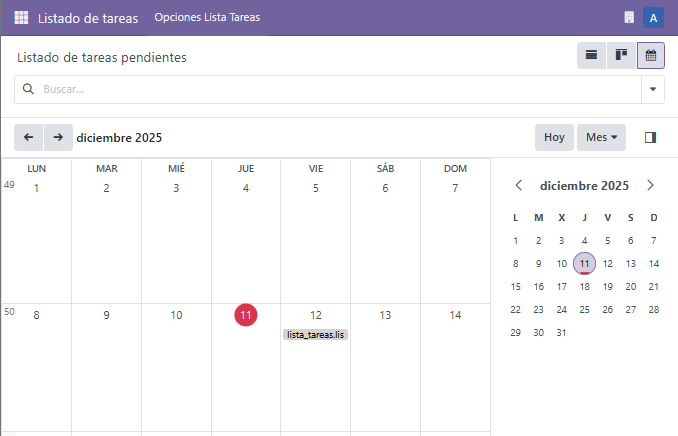
\includegraphics[width=0.8\textwidth]{Img/od11.png}
\end{figure}

\newpage
\volverindice
\begin{figure}[H]
\centering
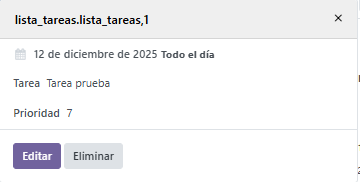
\includegraphics[width=0.6\textwidth]{Img/od12.png}
\end{figure}

Con la comprobación y confirmación de que todos los nuevos cambios realizados en el módulo \textbf{Lista\_Tareas} funcionan perfectamente, daremos por completada esta actividad.

\section{Actividad 02: Ampliación del Módulo Biblioteca}
En esta actividad, se nos indica realizar una ampliación del módulo añadiendo dos nuevas clases, así como sus restricciones correspondientes.

\subsection{Implementación de Socio}
La primera implementación que se nos pide es \textbf{crear la nueva clase Socio}, que almacenará los datos (\textbf{Nombre, Apellidos e Identificador}).

Para realizar esta implementación, desde el archivo \textbf{biblioteca\_comic.py} en \textbf{Models} crearemos la siguiente clase:

\begin{tcolorbox}[title=Nueva Clase Socio]
\begin{figure}[H]
\centering
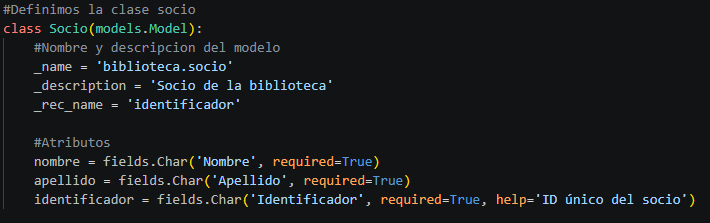
\includegraphics[width=1\textwidth]{Img/od16.0.png}
\end{figure}
\end{tcolorbox}

\newpage
\volverindice
\subsection{Implementación de Ejemplares}
Con la \textbf{clase Socio} implementada, a continuación crearemos la \textbf{clase Ejemplar} para gestionar los préstamos. Esta clase será la encargada de representar cada copia física de un cómic disponible para préstamo, relacionando cada ejemplar con el cómic original y con el socio que lo tenga en posesión en caso de estar prestado.

Para ello, añadiremos la siguiente clase en el archivo \textbf{biblioteca\_comic.py} dentro del módulo \textbf{Models}:

\begin{tcolorbox}[title=Nueva Clase Ejemplar]
\begin{figure}[H]
\centering
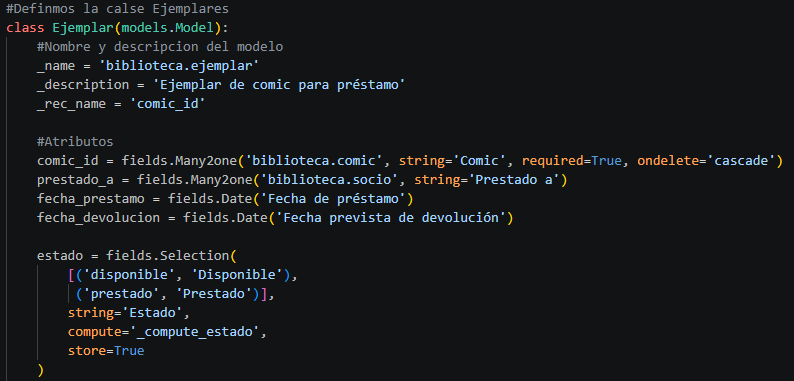
\includegraphics[width=1\textwidth]{Img/od16.1.png}
\end{figure}
\end{tcolorbox}

\subsubsection{Restricciones de fechas}
Una vez definida la clase, añadiremos unas \textbf{restricciones encargadas de controlar} que la fecha de préstamo no sea posterior al día actual, y que la fecha de devolución no sea anterior al día actual.

Para ello, añadimos el siguiente método:

\newpage
\volverindice
\begin{tcolorbox}[title=Restricciones del modelo Ejemplar]
\begin{figure}[H]
\centering
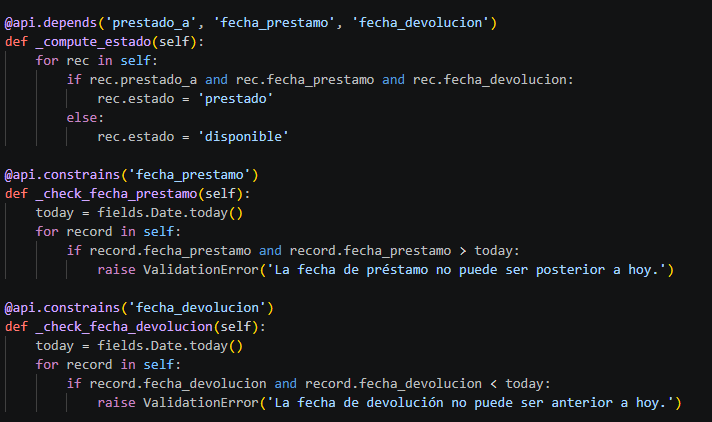
\includegraphics[width=1\textwidth]{Img/od16.2.1.png}
\end{figure}
\end{tcolorbox}

\subsubsection{Relación con el modelo Cómic}
Para finalizar con las restricciones, el modelo de cómic deberá estar relacionado con los ejemplares.

\begin{tcolorbox}[title=Relación con Cómic]
\begin{figure}[H]
\centering
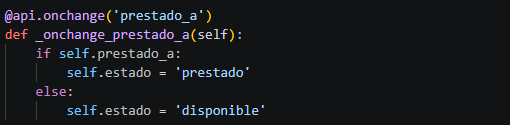
\includegraphics[width=1\textwidth]{Img/od16.2.0.png}
\end{figure}
\end{tcolorbox}

Con los nuevos códigos implementados, el archivo \textbf{biblioteca\_comic.py} quedará completo, lo que nos permitirá implementar los nuevos cambios necesarios en la sección de vistas.

\newpage
\volverindice
\subsection{Vistas y Menús}
Finalizada la implementación de las nuevas clases y sus restricciones correspondientes, nos dirigiremos al archivo \textbf{biblioteca\_comic.xml} en \textbf{Views} para definir las vistas, así como sus menús encargados de gestionar la información de cada una de forma clara.

\begin{tcolorbox}[title=Nueva Vista de Socio]
\begin{figure}[H]
\centering
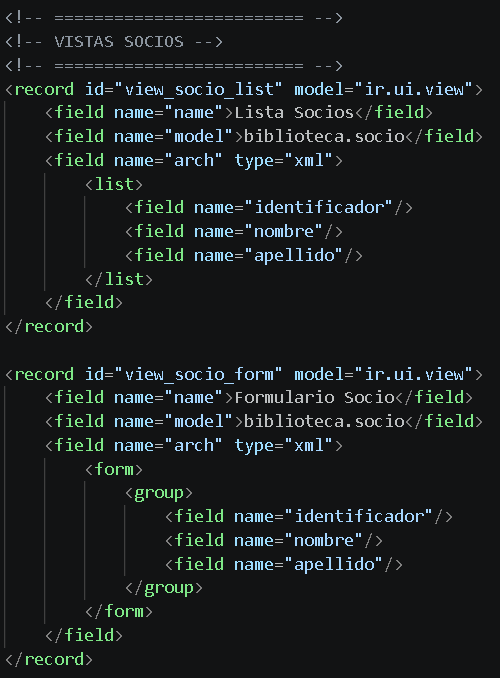
\includegraphics[width=0.8\textwidth]{Img/odo_vis_so.png}
\end{figure}
\end{tcolorbox}

\newpage
\volverindice
\begin{tcolorbox}[title=Nuevo Menú de Socio]
\begin{figure}[H]
\centering
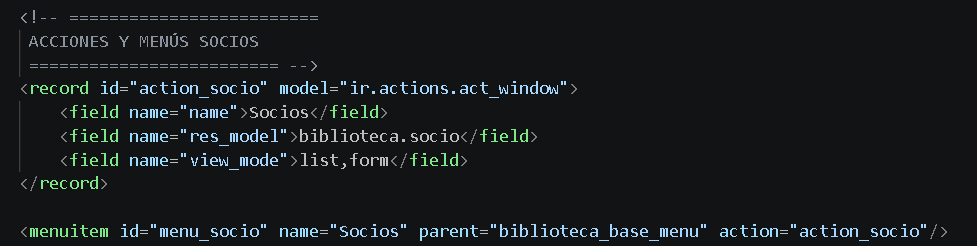
\includegraphics[width=1\textwidth]{Img/odo_menus.png}
\end{figure}
\end{tcolorbox}

\begin{tcolorbox}[title=Nueva Vista de Ejemplares]
\begin{figure}[H]
\centering
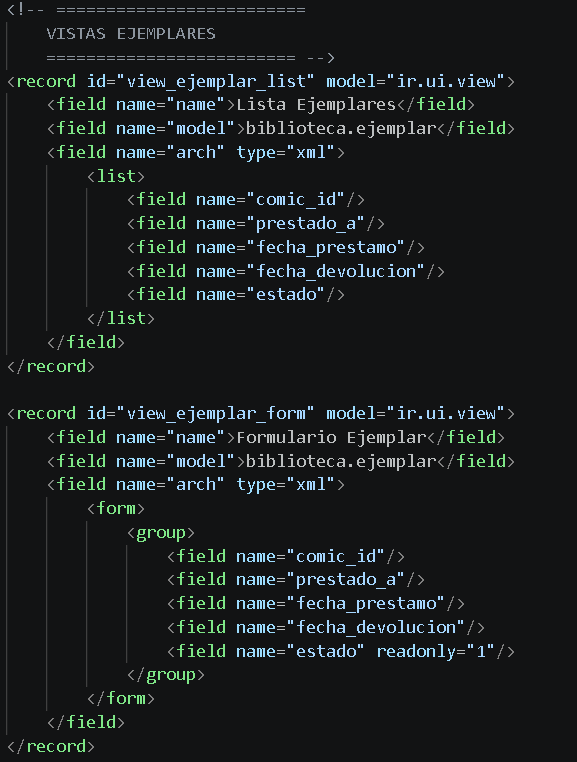
\includegraphics[width=0.7\textwidth]{Img/odo_eje_vis.png}
\end{figure}
\end{tcolorbox}

\newpage
\volverindice
\begin{tcolorbox}[title=Nuevo Menú de Ejemplares]
\begin{figure}[H]
\centering
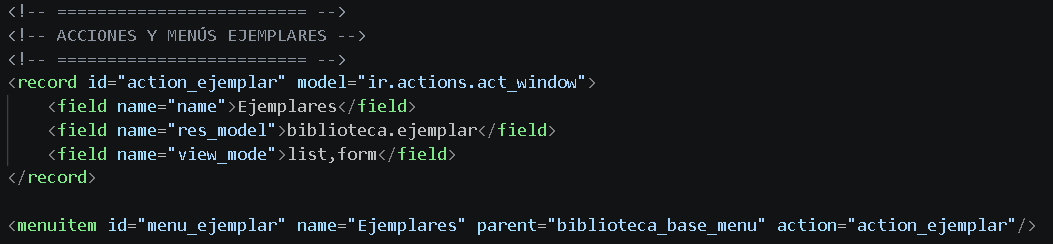
\includegraphics[width=1\textwidth]{Img/odo_me_ej.png}
\end{figure}
\end{tcolorbox}

Finalizada la implementación de las nuevas vistas y menús de forma correcta, realizaremos una comprobación desde Odoo para dar por finalizadas las nuevas modificaciones que se nos indican.

\subsection{Comprobación de Vistas}
Para realizar la comprobación, desde la sección de módulos instalados de nuestro Odoo, actualizaremos el módulo \textbf{Biblioteca Comics Simple}.

\begin{figure}[H]
\centering
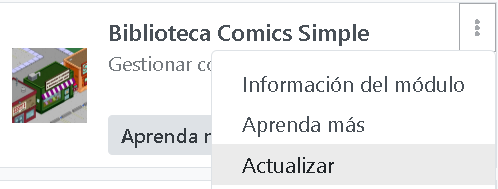
\includegraphics[width=0.7\textwidth]{Img/odo_bi_actu.png}
\end{figure}

Una vez realizada la actualización, ingresaremos al módulo desde el menú de aplicaciones.

\begin{figure}[H]
\centering
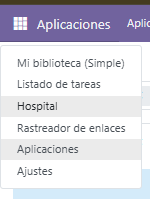
\includegraphics[width=0.3\textwidth]{Img/od18.png}
\end{figure}

\newpage
\volverindice
Lo primero que observaremos, en caso de que se haya realizado todo correctamente, son las vistas de los menús de navegación entre cómics, ejemplares y socios.

\begin{figure}[H]
\centering
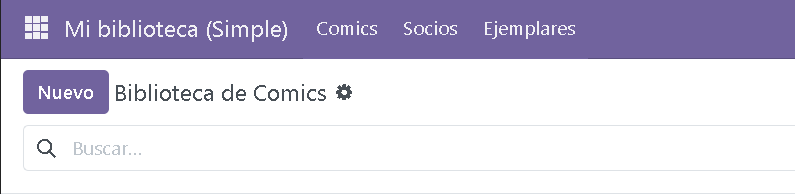
\includegraphics[width=1\textwidth]{Img/odo_compr.png}
\end{figure}

Dentro de la vista de \textbf{cómics}, podremos observar que se nos muestran los datos de forma correcta.

\begin{figure}[H]
\centering
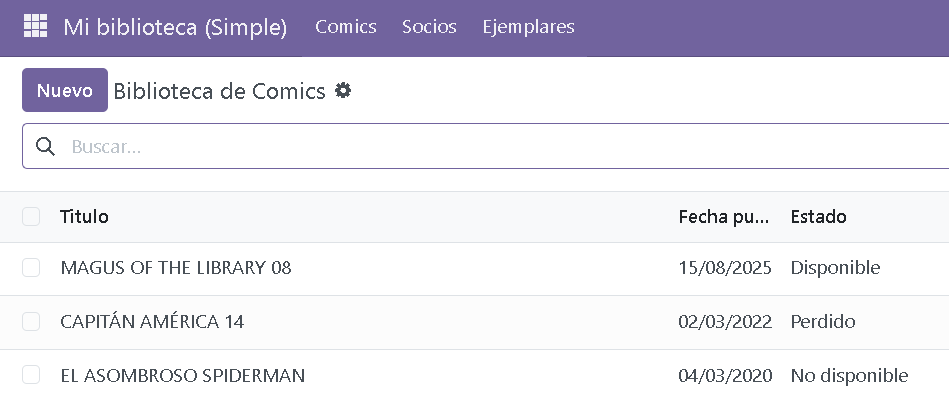
\includegraphics[width=1\textwidth]{Img/odo_com1.png}
\end{figure}

Así como en la vista de los \textbf{Socios}.

\begin{figure}[H]
\centering
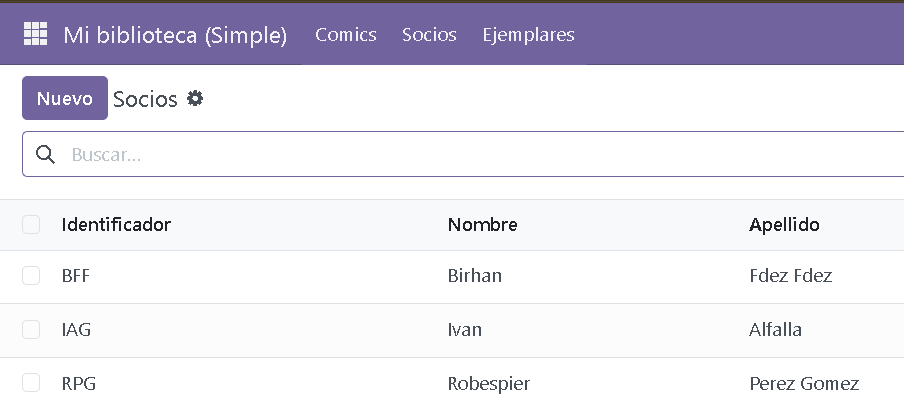
\includegraphics[width=1\textwidth]{Img/odo_com2.png}
\end{figure}

\newpage
\volverindice
Al crear un nuevo socio, podremos observar cómo, en caso de que no se ingrese todos los datos necesarios, el usuario recibirá una alerta de error.

\begin{figure}[H]
\centering
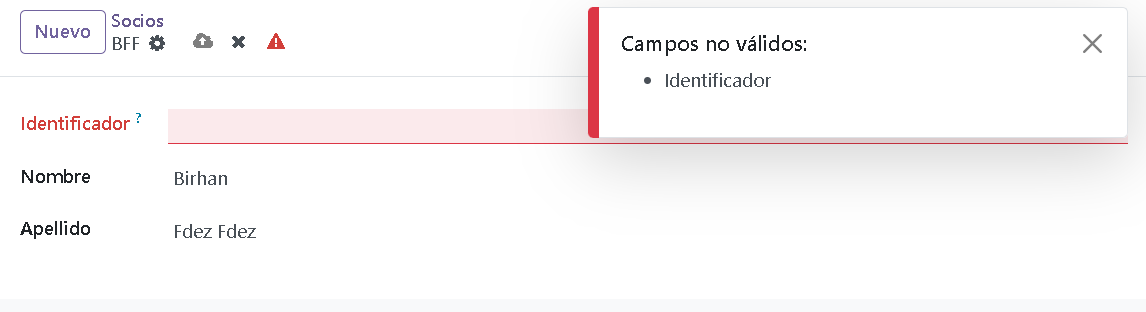
\includegraphics[width=1\textwidth]{Img/odo_com4.png}
\end{figure}

Seguido de la vista de \textbf{los ejemplares}.

\begin{figure}[H]
\centering
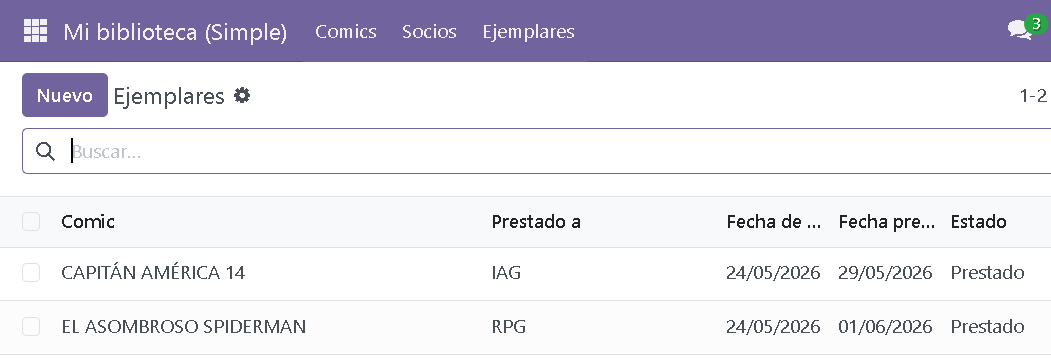
\includegraphics[width=1\textwidth]{Img/odo_com3.png}
\end{figure}

Donde podremos observar que, en caso de que el usuario introduzca una fecha de préstamo posterior a la fecha actual, este recibirá una alerta de error.

\begin{figure}[H]
\centering
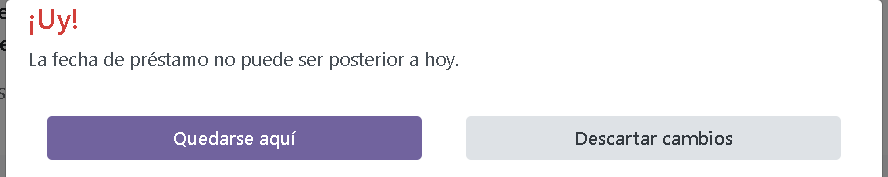
\includegraphics[width=1\textwidth]{Img/odo_com5.png}
\end{figure}

\newpage
\volverindice
Así como en caso de que la devolución sea en una fecha anterior a la del registro del préstamo.

\begin{figure}[H]
\centering
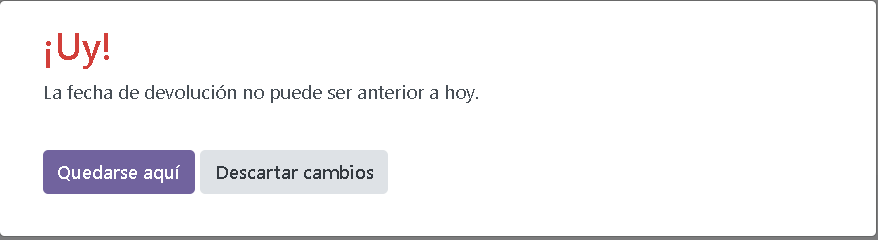
\includegraphics[width=0.7\textwidth]{Img/odo_com6.png}
\end{figure}

Con esto, podemos observar que las modificaciones que se nos piden en la actividad se cumplen y ejecutan de forma correcta, pudiendo así finalizar esta actividad.

\section{Actividad 03: Gestión Hospitalaria}
En esta actividad se nos indica crear un módulo de Odoo cuyas funciones son la gestión básica de un hospital. Este módulo tendrá que permitir la administración de pacientes, médicos y consultas.

\subsection{Paso Previo}
Para comenzar, lo primero que realizaremos es crear el módulo \textbf{Hospital} desde el Docker donde realizamos esta actividad. Esto lo podemos realizar empleando el siguiente código:

\begin{tcolorbox}[title=Comando Para Ingresar al Docker]
\begin{verbatim}
docker exec -it -u root e0.bigodoo.net /bin/bash
\end{verbatim}
\end{tcolorbox}

Una vez dentro de nuestro Docker, emplearemos este comando:

\begin{tcolorbox}[title=Comando Para Crear Módulo Básico]
\begin{verbatim}
odoo scaffold gestion_hospital /mnt/hospital_gestion
\end{verbatim}
\end{tcolorbox}

\begin{figure}[H]
\centering
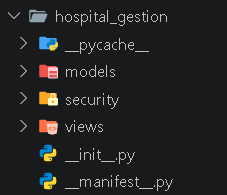
\includegraphics[width=0.4\textwidth]{Img/odo_crear_hospital.png}
\end{figure}

\newpage
\volverindice
Con el módulo básico creado, nos pondremos a trabajar en los elementos que se nos piden en la actividad.

\subsection{Modelos de Datos y Relaciones}
\subsubsection{Modelo Paciente}
Comenzaremos con el modelo del paciente. Para crear la clase de paciente, nos dirigimos al archivo \textbf{models.py} en la \textbf{sección de models}. Una vez dentro, crearemos la siguiente clase gestora con los atributos que se nos indican en la actividad.

\begin{tcolorbox}[title=Código Clase Paciente]
\begin{figure}[H]
\centering
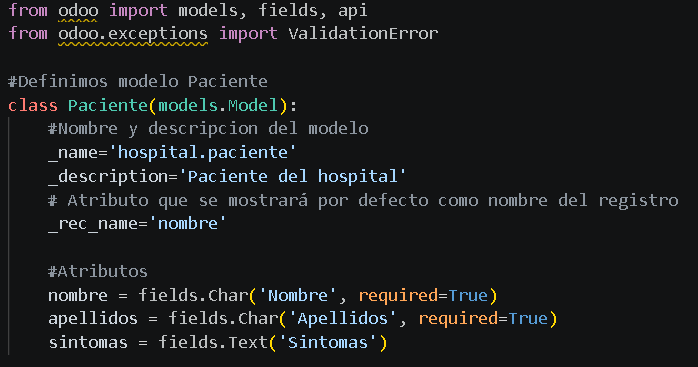
\includegraphics[width=1\textwidth]{Img/odo_hos_1.png}
\end{figure}
\end{tcolorbox}


\subsubsection{Modelo Médico}
Con la clase del paciente completada, lo siguiente que realizaremos es la creación de \textbf{la clase Médico}. Esta clase contendrá los atributos \textbf{Nombre, Apellidos y Número de colegiado}.

\begin{tcolorbox}[title=Código Clase Médico]
\begin{figure}[H]
\centering
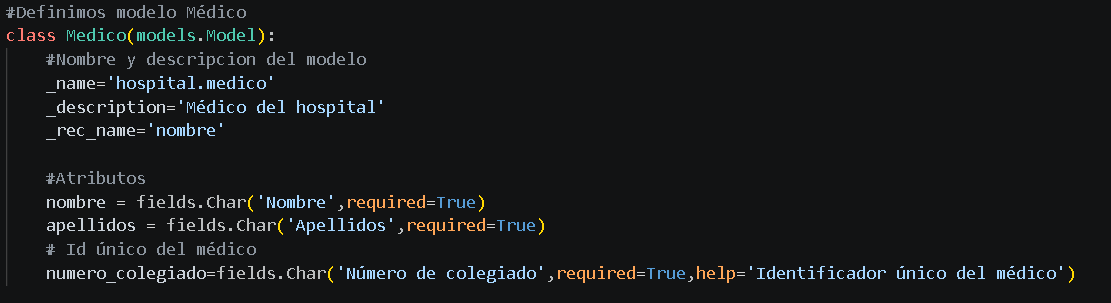
\includegraphics[width=1\textwidth]{Img/odo_hos_2.png}
\end{figure}
\end{tcolorbox}

\newpage
\volverindice
\subsubsection{Modelo Consulta}
Una vez finalizada la creación del módulo de médico, nos dispondremos a crear el módulo de \textbf{Consulta}. Antes de continuar, se debe tener en cuenta que este es el módulo principal, ya que en él se indican las relaciones entre las clases de médico y paciente. Una vez destacado esto, deberemos implementar el siguiente código.

\begin{tcolorbox}[title=Código Clase Consulta]
\begin{figure}[H]
\centering
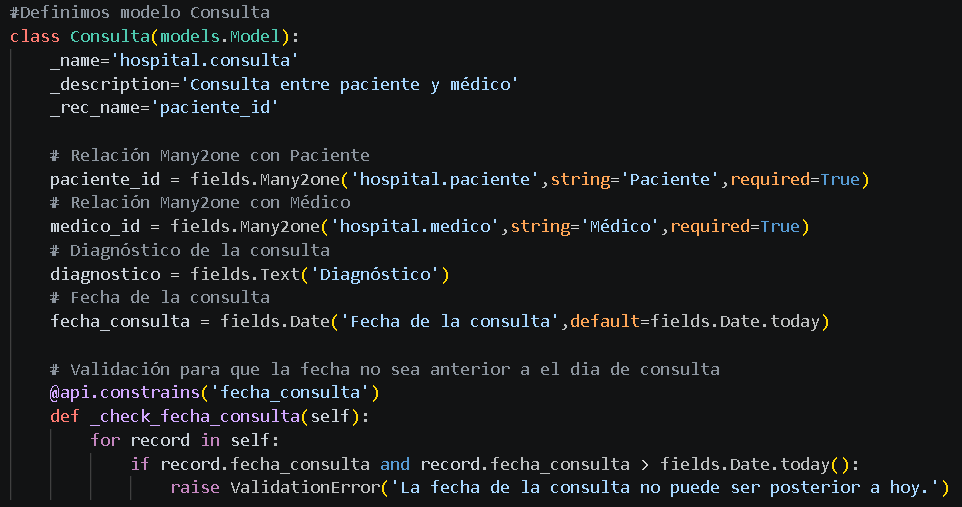
\includegraphics[width=1\textwidth]{Img/odo_hos_3.png}
\end{figure}
\end{tcolorbox}

Tras completar el código de la clase \textbf{consulta}, nos dirigiremos a la sección de vistas para completar la actividad.

\subsection{Vistas y Menús}
En este apartado de la actividad, nos dispondremos a codificar el formato de las vistas, así como el menú de navegación que permitirá al usuario moverse entre cada una de las gestiones.

Para comenzar, en la carpeta \textbf{Views} crearemos el archivo \textbf{hospital\_views.xml}. Con el archivo creado, implementaremos las vistas y los menús que permitirán a los usuarios interactuar con el módulo.

\newpage
\volverindice
\begin{tcolorbox}[title=Código Vista Paciente]
\begin{figure}[H]
\centering
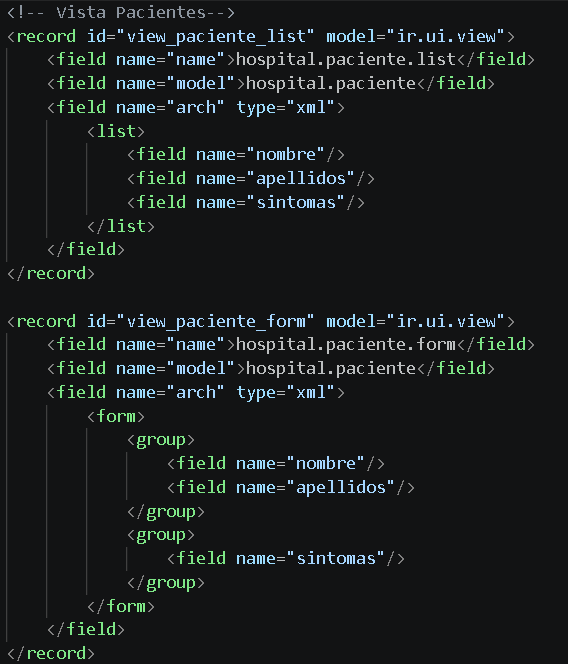
\includegraphics[width=0.8\textwidth]{Img/odo_hos_4.png}
\end{figure}
\end{tcolorbox}

\newpage
\volverindice
\begin{tcolorbox}[title=Código Vista Médico]
\begin{figure}[H]
\centering
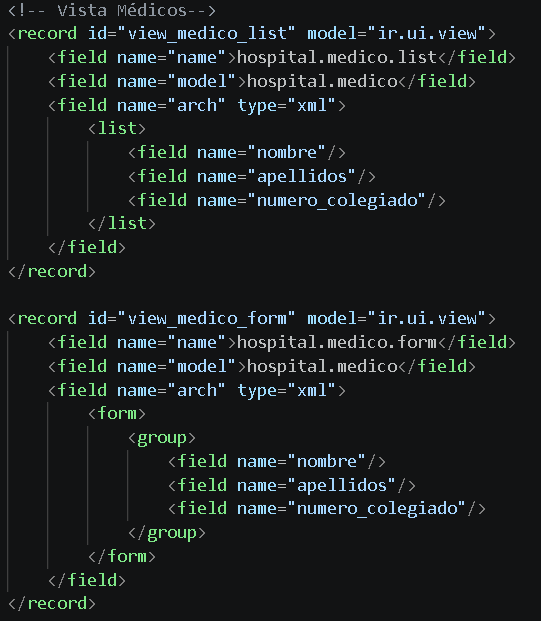
\includegraphics[width=0.7\textwidth]{Img/odo_hos_5.png}
\end{figure}
\end{tcolorbox}

\newpage
\volverindice
\begin{tcolorbox}[title=Código Vista Consulta]
\begin{figure}[H]
\centering
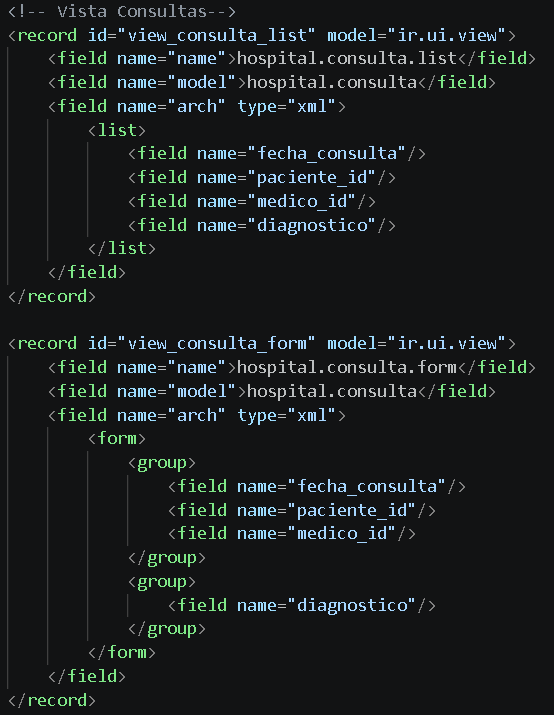
\includegraphics[width=0.7\textwidth]{Img/odo_hos_6.png}
\end{figure}
\end{tcolorbox}

\newpage
\volverindice
\begin{tcolorbox}[title=Código Menús de Navegación]
\begin{figure}[H]
\centering
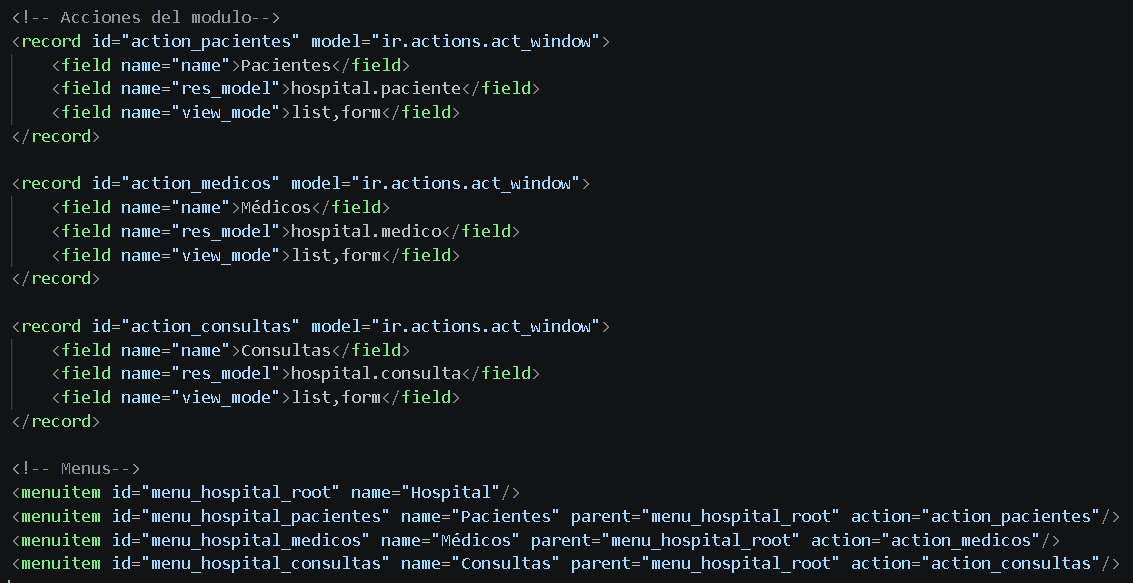
\includegraphics[width=1\textwidth]{Img/odo_hos_7.png}
\end{figure}
\end{tcolorbox}

Con las vistas y los menús correspondientes implementados de forma correcta, a continuación realizaremos una prueba de comprobación para confirmar el correcto funcionamiento del módulo.

\subsection{Comprobación de Vistas}
Para iniciar esta comprobación, debemos reiniciar nuestro Docker para que Odoo pueda aplicar los nuevos cambios y añadir el nuevo módulo.

Una vez completado el reinicio, empleando la barra de búsqueda ingresaremos el nombre de nuestro módulo para poder instalarlo y comenzar a interactuar con él.

\begin{figure}[H]
\centering
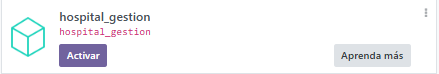
\includegraphics[width=1\textwidth]{Img/od17.png}
\end{figure}

\newpage
\volverindice
Con el módulo operativo, ingresaremos y realizaremos una prueba creando un paciente, un médico y una consulta.

\begin{figure}[H]
\centering
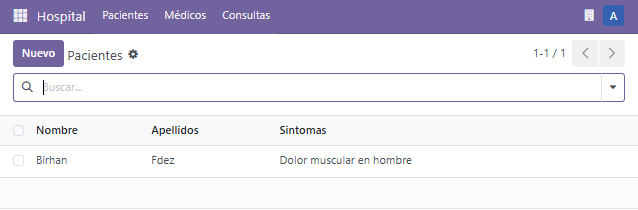
\includegraphics[width=1\textwidth]{Img/od19.png}
\end{figure}

\begin{figure}[H]
\centering
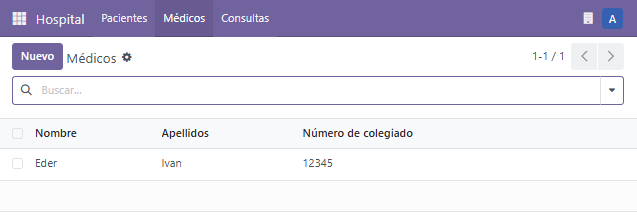
\includegraphics[width=1\textwidth]{Img/od20.png}
\end{figure}

\begin{figure}[H]
\centering
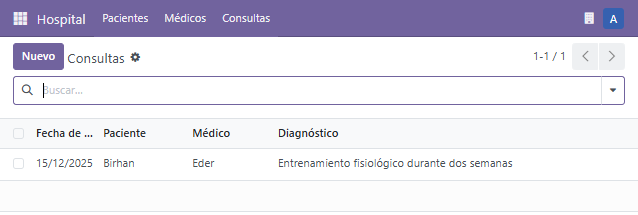
\includegraphics[width=1\textwidth]{Img/od21.png}
\end{figure}

Si la implementación del módulo se realizó de forma correcta y no se detectó ningún fallo, podremos dar por concluida esta actividad.

\newpage
\volverindice
\section{Actividad 04: Gestión de Ciclos Formativos}
En esta actividad, se nos indica crear un módulo cuya función es \textbf{la gestión de ciclos formativos, módulos, alumnos y profesores} en un instituto. Para ello, emplearemos el mismo método que se usó en el módulo de la actividad anterior.

\begin{tcolorbox}[title=Comandos Para Ingresar al Docker y Crear el Módulo Básico]
\begin{verbatim}
# Comando Ingreso a Docker
docker exec -it -u root e0.bigodoo.net /bin/bash

# Comando Creación Módulo Básico
odoo scaffold ciclos_formativos /mnt/ciclos_formativos
\end{verbatim}
\end{tcolorbox}

Una vez ejecutados estos comandos, el usuario observará la aparición de una nueva carpeta llamada \textbf{ciclos\_formativos}, donde realizará la creación e implementación de los modelos, así como de sus vistas y la configuración de los permisos.

\begin{figure}[H]
\centering
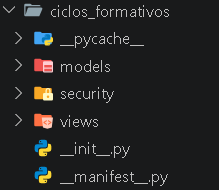
\includegraphics[width=0.4\textwidth]{Img/odo_cicl01.png}
\end{figure}

\newpage
\volverindice
\subsection{Modelos de Datos y Relaciones}
\subsubsection{Modelo Ciclo Formativo}
En esta sección nos disponemos a desarrollar el modelo de ciclo formativo, donde implementaremos sus atributos, así como su nombre y descripción.

\begin{tcolorbox}[title=Código Modelo Ciclos Formativos]
\begin{figure}[H]
\centering
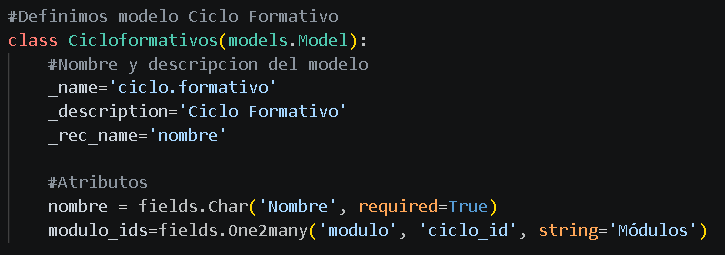
\includegraphics[width=1\textwidth]{Img/odo_cicl02.png}
\end{figure}
\end{tcolorbox}

\subsubsection{Modelo Módulo}
A continuación se muestra el código de la clase \textbf{Módulo}, que gestionará los módulos con los que contará el ciclo. En él se puede observar que este módulo está relacionado con los ciclos, los profesores y los alumnos.

\begin{tcolorbox}[title=Código Modelo Módulo]
\begin{figure}[H]
\centering
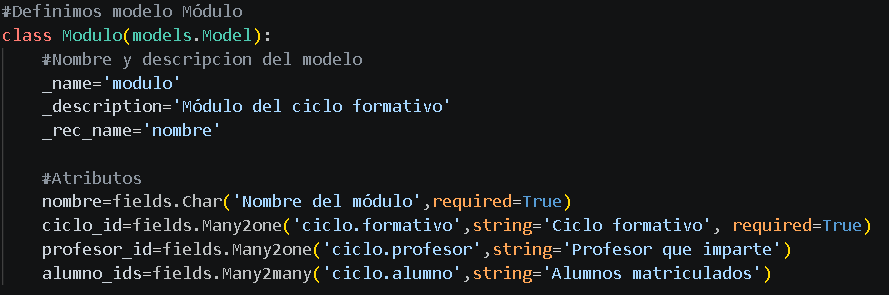
\includegraphics[width=1\textwidth]{Img/odo_cicl03.png}
\end{figure}
\end{tcolorbox}

\newpage
\volverindice
\subsubsection{Modelo Alumno}
En el código que se muestra a continuación, se muestra la implementación del modelo de alumnos con sus atributos correspondientes, así como sus relaciones.

\begin{tcolorbox}[title=Código Modelo Alumno]
\begin{figure}[H]
\centering
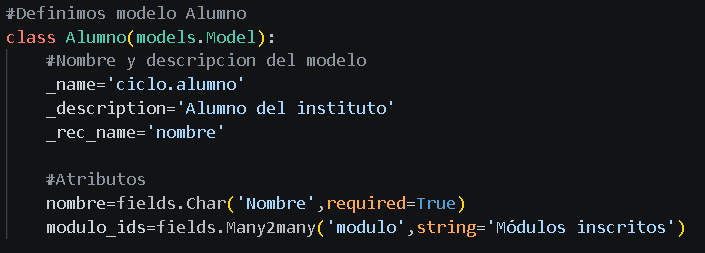
\includegraphics[width=1\textwidth]{Img/odo_cicl04.png}
\end{figure}
\end{tcolorbox}

\subsubsection{Modelo Profesor}
En este apartado implementamos la clase \textbf{Profesor}.

\begin{tcolorbox}[title=Código Modelo Profesor]
\begin{figure}[H]
\centering
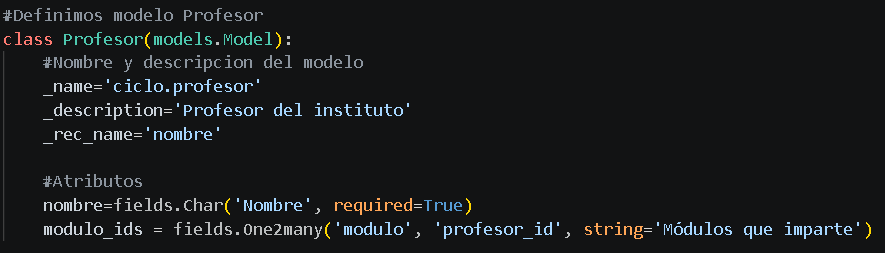
\includegraphics[width=1\textwidth]{Img/odo_cicl05.png}
\end{figure}
\end{tcolorbox}

Con todo lo anterior finalizado, nos podremos dirigir a la sección de vistas, donde codificaremos las vistas del módulo, así como su menú.

\subsection{Vistas y Menús}
Con los modelos implementados, a continuación implementaremos las vistas con las que interactuará el usuario.

Para comenzar, lo primero que implementaremos será la vista de ciclos.

\newpage
\volverindice
\begin{tcolorbox}[title=Código Vista Ciclos]
\begin{figure}[H]
\centering
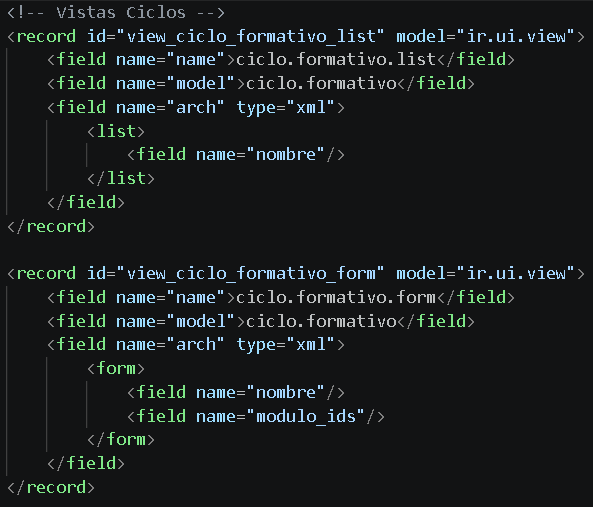
\includegraphics[width=0.6\textwidth]{Img/odo_cicl06.png}
\end{figure}
\end{tcolorbox}

Seguido de la vista de módulo.

\begin{tcolorbox}[title=Código Vista Módulo]
\begin{figure}[H]
\centering
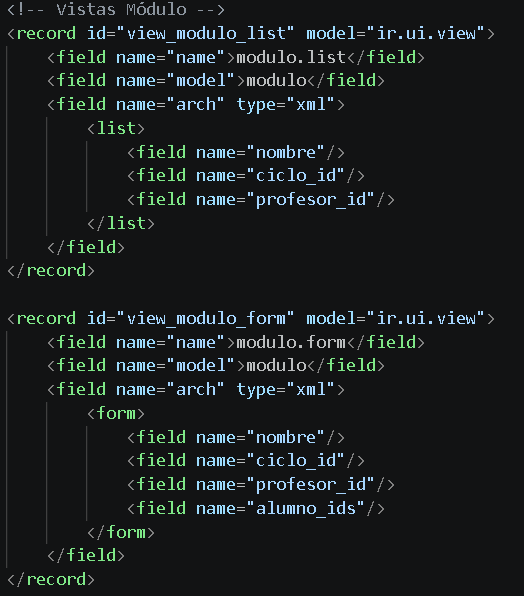
\includegraphics[width=0.6\textwidth]{Img/odo_cicl07.png}
\end{figure}
\end{tcolorbox}

La vista de Alumno.

\begin{tcolorbox}[title=Código Vista Alumno]
\begin{figure}[H]
\centering
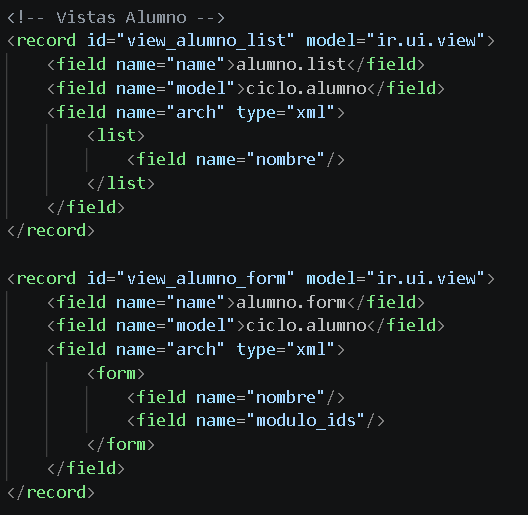
\includegraphics[width=0.6\textwidth]{Img/odo_cicl08.png}
\end{figure}
\end{tcolorbox}

Y por último, la vista de Profesor.

\begin{tcolorbox}[title=Código Vista Profesor]
\begin{figure}[H]
\centering
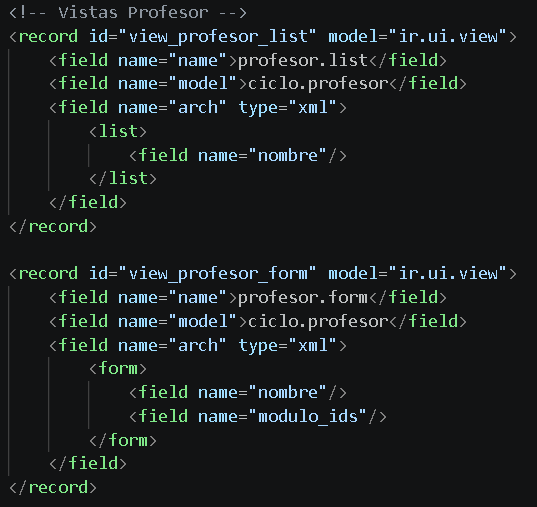
\includegraphics[width=0.6\textwidth]{Img/odo_cicl09.png}
\end{figure}
\end{tcolorbox}

\newpage
\volverindice
Con las vistas finalizadas, a continuación implementaremos los menús y las acciones correspondientes para poder navegar entre cada uno de los modelos.

\begin{tcolorbox}[title=Código Acciones y Menús]
\begin{figure}[H]
\centering
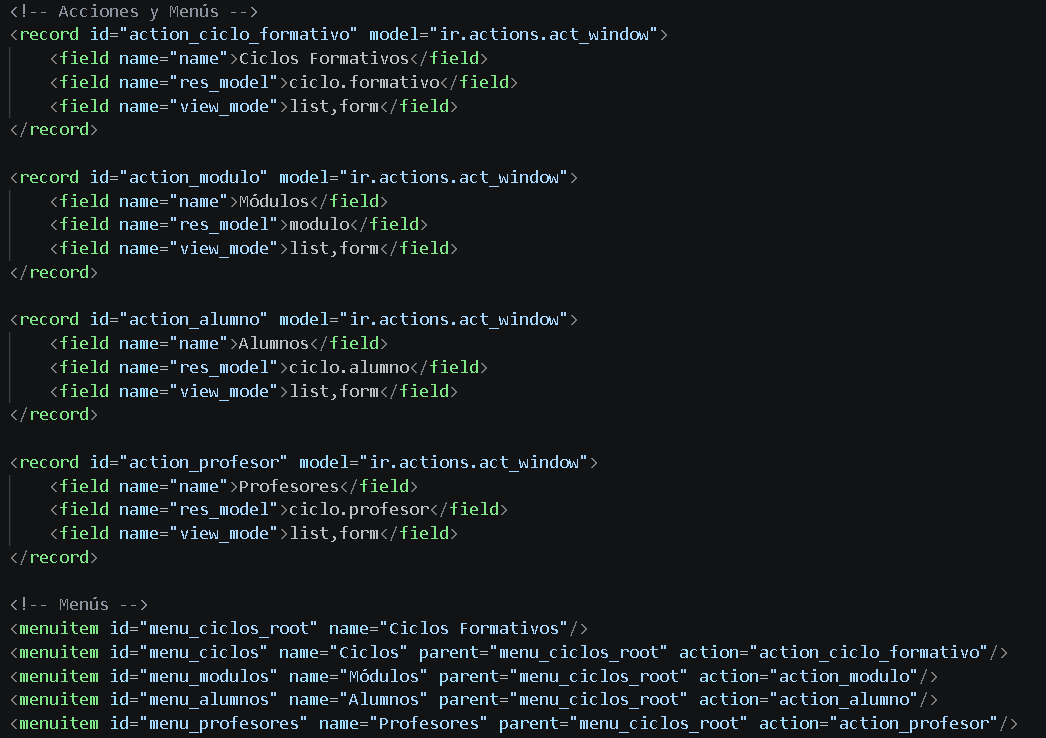
\includegraphics[width=1\textwidth]{Img/odo_cicl10.png}
\end{figure}
\end{tcolorbox}

\subsection{Comprobación de Vistas}
Con las vistas y los menús de interacción implementados, a continuación realizaremos una comprobación para observar que todo el módulo opera correctamente.

Para ello, buscaremos nuestro módulo y lo instalaremos.

\begin{figure}[H]
\centering
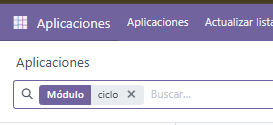
\includegraphics[width=0.7\textwidth]{Img/od22.png}
\end{figure}

\newpage
\volverindice
\begin{figure}[H]
\centering
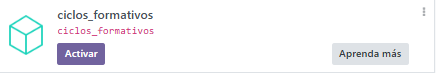
\includegraphics[width=0.7\textwidth]{Img/od23.png}
\end{figure}

Una vez completada la instalación, ingresaremos al módulo para comprobar su correcto funcionamiento.

Lo primero que realizaremos será la creación de un par de ciclos, así como alumnos y profesores, para luego implementar los módulos con los datos que se necesitan.

\begin{tcolorbox}[title=Vista Ciclos]
\begin{figure}[H]
\centering
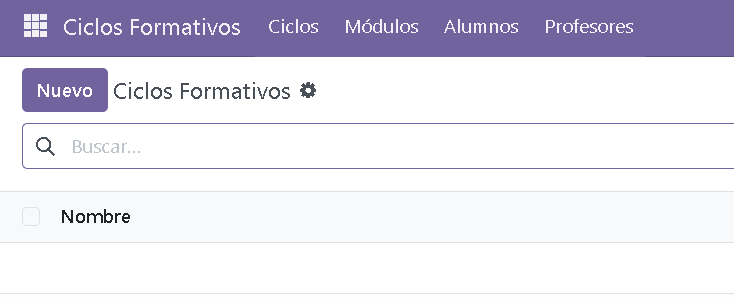
\includegraphics[width=0.9\textwidth]{Img/odo_cicl14.png}
\end{figure}
\end{tcolorbox}

\begin{tcolorbox}[title=Vista Ciclos con ciclos implementados]
\begin{figure}[H]
\centering
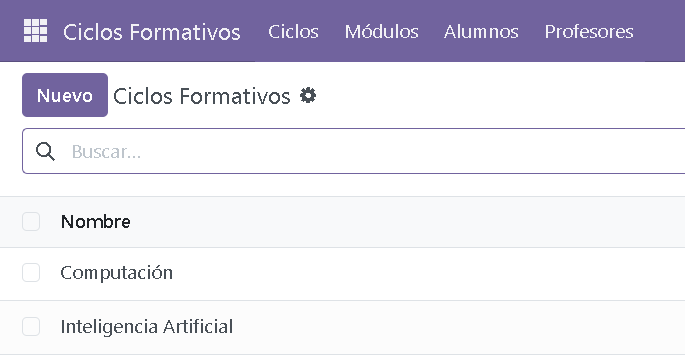
\includegraphics[width=0.9\textwidth]{Img/odo_cicl15.png}
\end{figure}
\end{tcolorbox}

\newpage
\volverindice
\begin{tcolorbox}[title=Vista Alumnos]
\begin{figure}[H]
\centering
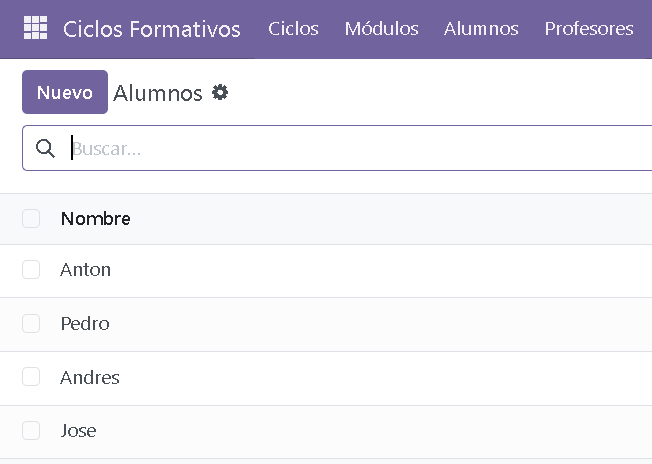
\includegraphics[width=0.9\textwidth]{Img/odo_cicl16.png}
\end{figure}
\end{tcolorbox}

\begin{tcolorbox}[title=Vista Profesores]
\begin{figure}[H]
\centering
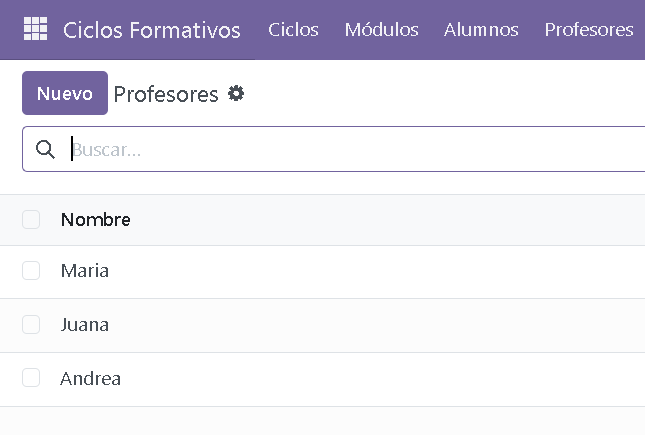
\includegraphics[width=0.9\textwidth]{Img/odo_cicl17.png}
\end{figure}
\end{tcolorbox}

\newpage
\volverindice
\begin{tcolorbox}[title=Vista Módulos]
\begin{figure}[H]
\centering
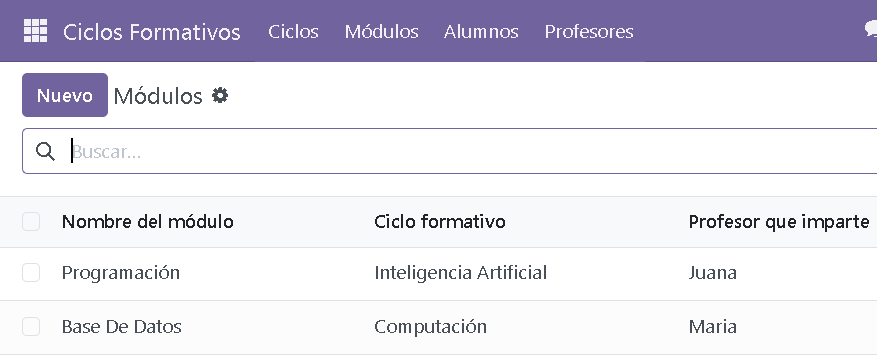
\includegraphics[width=0.9\textwidth]{Img/odo_cicl18.png}
\end{figure}
\end{tcolorbox}

\begin{tcolorbox}[title=Vista Módulo con su profesor y alumnos matriculados]
\begin{figure}[H]
\centering
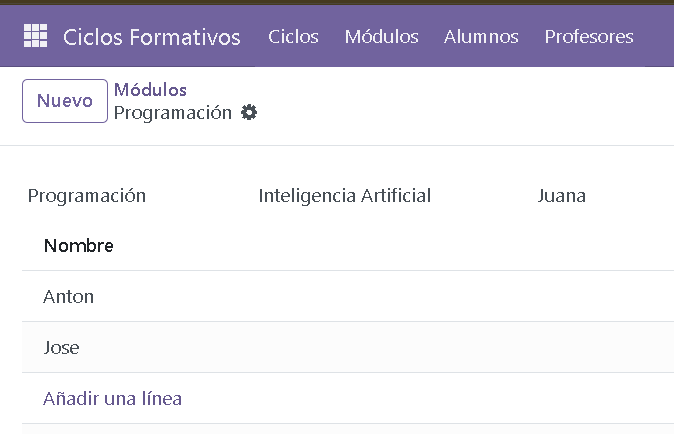
\includegraphics[width=0.9\textwidth]{Img/odo_cicl19.png}
\end{figure}
\end{tcolorbox}

\newpage
\volverindice
\subsection{Configuración de seguridad}
Tras confirmar el correcto funcionamiento del módulo, a continuación nos dispondremos a implementar unas configuraciones de seguridad.

Para ello, nos dirigimos a la carpeta \textbf{security}, donde crearemos un nuevo archivo llamado \textbf{groups.xml} para crear los grupos de seguridad que contendrán los privilegios.

Con el archivo creado, a continuación implementaremos el siguiente código que gestionará los usuarios por grupos.

\begin{tcolorbox}[title=Roles de los Usuarios]
\begin{figure}[H]
\centering
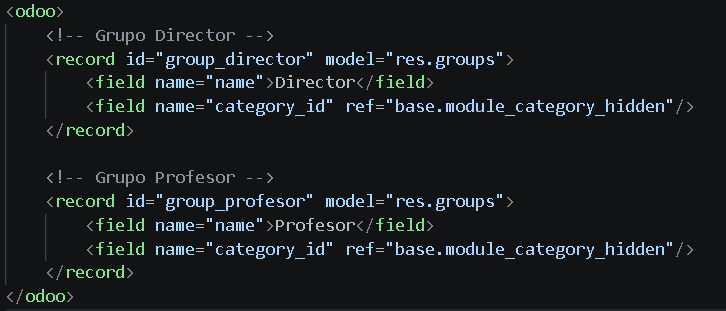
\includegraphics[width=1\textwidth]{Img/odo_cicl12.png}
\end{figure}
\end{tcolorbox}

Una vez creados los grupos, nos dirigiremos al archivo \textbf{ir.model.access.csv}, donde indicaremos los permisos que obtendrá cada uno.

En la actividad se nos indica que los usuarios con el rol de \textbf{Director} podrán modificar los registros de los modelos anteriores, mientras que los usuarios con el rol de \textbf{Profesor} serán los únicos que podrán ver los datos de los profesores (en modo lectura).

Para ello implementaremos el siguiente código de permisos:

\begin{tcolorbox}[title=Permisos de acceso]
\begin{figure}[H]
\centering
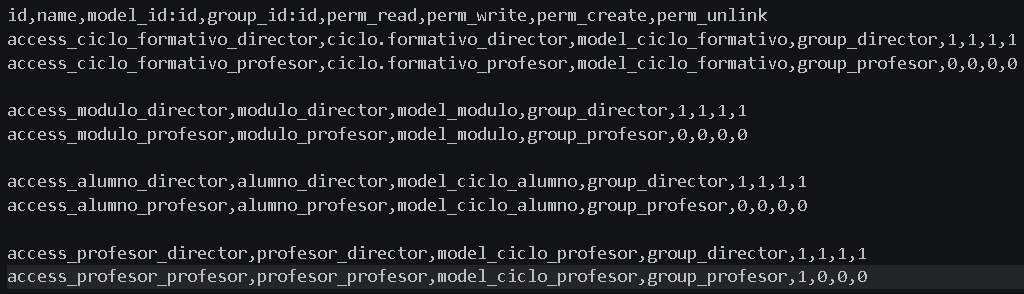
\includegraphics[width=1\textwidth]{Img/odo_cicl13.png}
\end{figure}
\end{tcolorbox}

\newpage
\volverindice
\subsection{Comprobación de permisos}
Para verificar que la configuración de seguridad funciona correctamente, asignamos los permisos correspondientes a cada usuario.

\begin{tcolorbox}[title=Permisos de acceso de Director]
\begin{figure}[H]
\centering
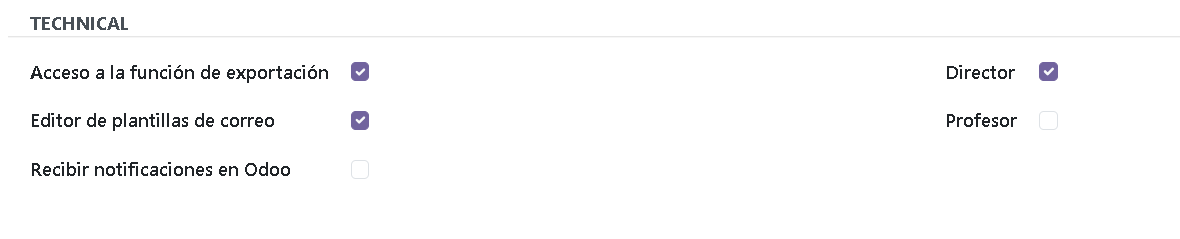
\includegraphics[width=1\textwidth]{Img/odo_cicl22.png}
\end{figure}
\end{tcolorbox}

\begin{tcolorbox}[title=Comprobación de Permisos de acceso de Director]
\begin{figure}[H]
\centering
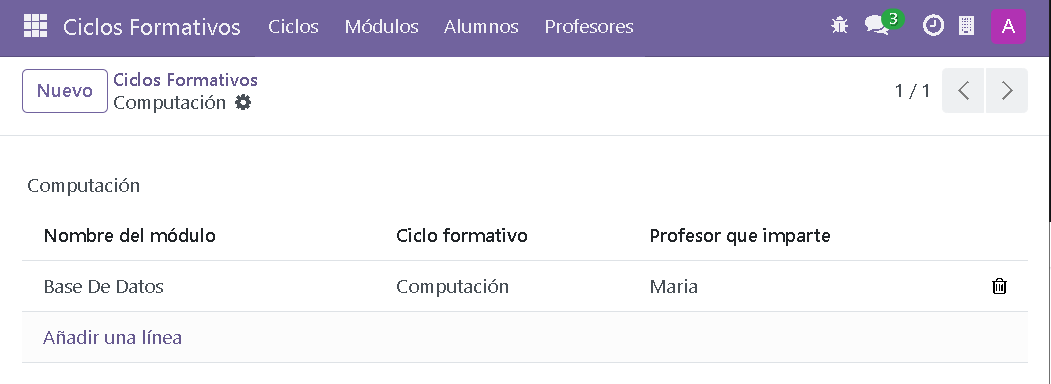
\includegraphics[width=1\textwidth]{Img/odo_cicl24.png}
\end{figure}
\end{tcolorbox}

\begin{tcolorbox}[title=Permisos de acceso de Profesor]
\begin{figure}[H]
\centering
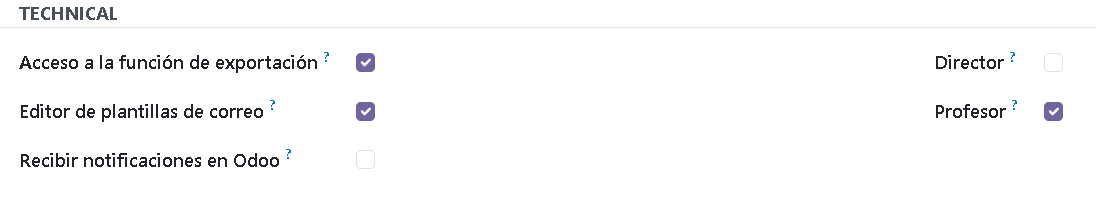
\includegraphics[width=1\textwidth]{Img/odo_cicl25.png}
\end{figure}
\end{tcolorbox}

\begin{tcolorbox}[title=Comprobación de Permisos de acceso de Profesor]
\begin{figure}[H]
\centering
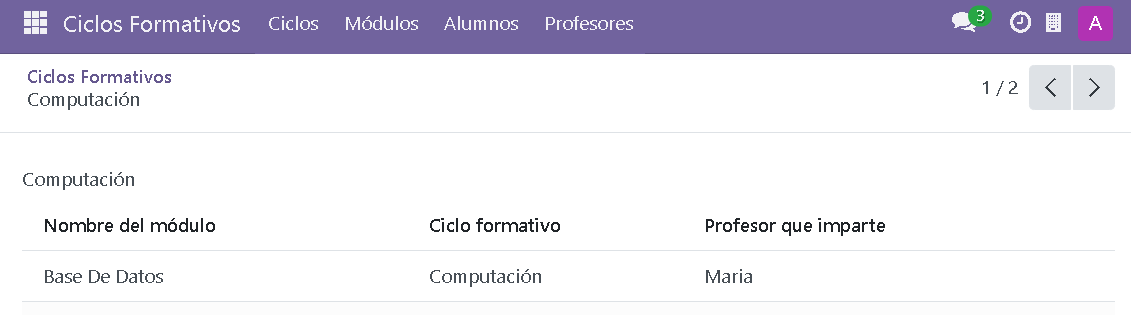
\includegraphics[width=1\textwidth]{Img/odo_cicl23.png}
\end{figure}
\end{tcolorbox}

Como se puede observar:
\begin{itemize}
    \item El usuario con rol \textbf{Director} tiene permisos completos sobre todos los modelos (lectura, escritura, creación y eliminación).
    \item El usuario con rol \textbf{Profesor} solo tiene permiso de lectura sobre el modelo de profesores.
\end{itemize}

Con esta comprobación final de los permisos de seguridad finalizado, podremos da por concluido la actividad así como la prelaticia.

\end{document}